Se pretende dar solución mediante un proyecto informático a una problemática real que actualmente se está solucionando mediante trámites gestionados vía telefónica. Inicialmente se observa un problema cercano localizado en algún organismo público y que pueda ser escalable. La búsqueda de un problema al cuál dar solución se inicia en la localidad en la que reside el autor de este proyecto. \\

Día a día, se puede observar que hay una tendencia creciente al reciclaje tanto de muebles como de electrodomésticos. Según estudios \cite{AndaluciaEcologica:web} llevados a cabo por la Consejería de Medio Ambiente de la Junta de Andalucía: se observa que desde el año 1999 al 2008 se produjo un considerable incremento en la cantidad de Plantas de clasificación, recuperación, transferencia y vertederos de apoyo; por otro lado se redujeron bastante los vertederos de residuos no peligrosos. Todo ello nos lleva a observar una considerable inversión por parte de la comunidad autónoma de Andalucía por el reciclaje. Por otra parte también de dicho estudio se puede sacar la conclusión de que hay un mayor indice generalizado de residuos por habitante tal y como se observa en la gráfica, y que es una tendencia de todas las provincias de la comunidad autónoma de Andalucía. Si revisamos el \textit{Plan Director Territorial de Residuos No Peligrosos}\cite{conserjeria_de_medio_ambiente_junta_de_andalucia_plan_2011} redactado por el Consejo de Gobierno de la Junta de Andalucía en el 2011, en lo referido a la recogida de aparatos eléctricos y electrodomésticos hay un considerable crecimiento en el número de electrodomésticos depositados como residuos, y se prevé una duplicación de dicho demanda en 12 años. Adicionalmente, se indica que el 89\% de ellos proceden de hogares particulares, y destaca el incremento de plantas dedicadas al tratamiento de dichos residuos. Se deja claro que la recogía de dichos enseres será gestionado por cada uno de los ayuntamientos. \\

De todo lo anterior, se puede observar un incremento de puntos limpios y una mayor organización de los residuos depositados. Se puede concluir, que durante los últimos años se ha ido incrementando considerablemente el número de residuos voluminosos depositados en cada uno de los municipios, esto se debe principalmente a la cada vez mayor tendencia a renovación de muebles o electrodomésticos y a la rotura o avería de estos. \\

\begin{figure}[H]
\begin{center}
    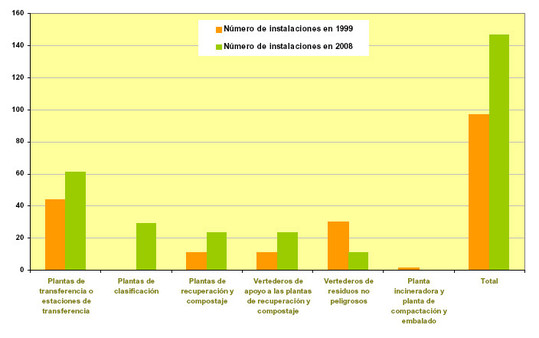
\includegraphics[scale=0.60]{grafica-plantas-residuos.jpg}
\end{center}
    \caption{Infraestructura para la gestión de residuos domiciliarios (1999-2008). Fuente: Borrador Plan Director Territorial de Residuos no peligrosos de Andalucía 2010-2019}
\end{figure}

\begin{figure}[H]
\begin{center}
    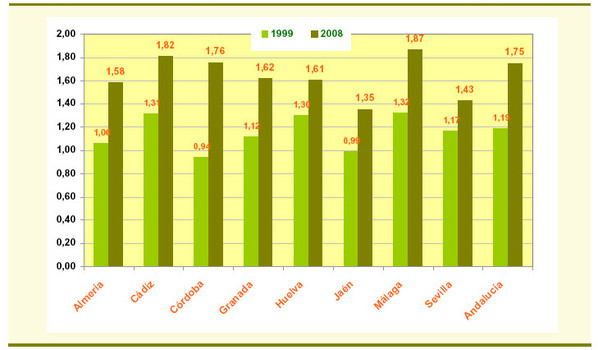
\includegraphics[scale=0.60]{grafica-residuos-habitante.jpg}
\end{center}
    \caption{Evolución de la generación de Residuos Urbanos 1999-2008 (Kg./hab/día). Fuente: Borrador Plan Director Territorial de Residuos no peligrosos de Andalucía 2010-2019}
\end{figure}

La operativa habitual a la hora de gestionar la recogida de dichos residuos es bastante similar en unos u otros municipios. Para informarnos de cómo se suele realizar la tramitación de la recogida de enseres se han consultado empresas municipales de la zona, a continuación se muestra una tabla con la información obtenida. \\

% Tabla de estado actual del servicio de recogida de enseres.
\begin{sidewaystable}
    \centering
\begin{tabular}{|c|l|ll}
\cline{1-2}
\textbf{Localidad}       & \multicolumn{1}{|c|}{\textbf{Operativa}}                                                                                                                    &  \\ \cline{1-2}
Cádiz                    & \begin{tabular}[c]{@{}c@{}}previa petición de los mismos al teléfono 956 262611\\ de lunes a viernes.\end{tabular}                                          &               \\ \cline{1-2}
El Puerto de Santa María & previa petición de los mismos al teléfono 900 102 697                                                                                                       &              \\ \cline{1-2}
Puerto Real              & previa petición de los mismos al teléfono 956474448                                                                                                         &              \\ \cline{1-2}
San Fernando             & \begin{tabular}[c]{@{}c@{}}previa petición de los mismos al teléfono 956 880 884 o bien \\ solicitud web mediante portal web del ayuntamiento.\end{tabular} &              &  \\ \cline{1-2}
Jerez de la frontera     & \begin{tabular}[c]{@{}c@{}}Recogida nocturna por zonas, no requiere petición previa, pero \\  sí informarse de que día se recoge en cada zona al teléfono gratuito 010.\end{tabular} &              \\ \cline{1-2}
\end{tabular}
\caption{Operativas de recogida de enseres de ayuntamientos consultados}
\end{sidewaystable}

Actualmente lo general es ofrecer la realización de dicho servicio de recogida mediante un número de teléfono gratuito puesto a disposición de la ciudadanía. A pesar de ello, hay un cierto desconocimiento por parte de ésta de en qué consiste el servicio y qué trámites hay que llevar a cabo para solicitar la recogida: prueba de ello es que, en el término de Puerto Real sólo el 40\% de las intervenciones de recogida fueron realizadas el año pasado por aviso de los usuarios \cite{articulo:lavozdecadiz}. Se hace necesario tanto promover una mayor cultura de reciclaje, como facilitar y dar una mayor comodidad a los trámites para solicitar la recogida de enseres. Se trata pues de buscar un medio alternativo al número de teléfono gratuito con horario específico de atención al cliente y un único operador tramitando una tras otra peticiones de similar tipología. \\

Inicialmente se barajan dos posibles soluciones, por un lado ofrecer una aplicación web que gestione ese tipo de peticiones y por otro una aplicación para terminales \textit{
smartphone}. Según el informe \textit{The Digitar Consumer} \cite{the_nielsen_company_digital_2014}, se puede observar que cada vez se utilizan más los dispositivos móviles para navegar por internet y realizar diversas gestiones. De media, los usuarios pasan más 34 horas y 17 minutos al mes con su terminal smartphone navegando por internet o utilizando aplicaciones, mientras que haciendo uso del ordenador y realizando esas mismas tareas pasan de media 27 horas y 3 minutos mensuales. Es por ello que para llegar a un mayor número de usuarios, y dada esta tendencia actual, interesa ofrecer la solución al problema planteado mediante la oferta de una alternativa que permita realizar dicha gestión mediante una aplicaciones disponible desde teléfono móvil. \\

De entre las diversas plataformas móviles existente interesará la mayormente usada en España, ya que interesa maximizar la difusión de la aplicación y de esta forma llegar al máximo número de ciudadanos. Durante el mes de febrero del 2014 según un estudio realizado por \textit{Kantar WordPanel} \cite{kantar_wordpanel_publications_2014} se observa que la plataforma de mayor difusión en nuestro país es Android con un 86\% de cuota de mercado. Por lo tanto se opta por ofrecer una funcionalidad rutinaria que a día de hoy se está llevando a cabo vía telefónica hablando con un operador mediante una aplicación móvil para la plataforma de mayor difusión que en este caso es \textit{Android}.\\

\begin{figure}[H]
\begin{center}
    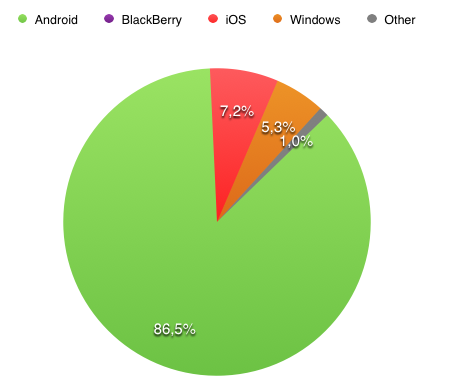
\includegraphics[scale=0.60]{estudio-plataformas.png}
\end{center}
    \caption{Smartphone OS market share España (febrero del 2014)}
\end{figure}
